This is draft of large paper that Jack started.

\section{\label{sec.PFF_Intro}Introduction}

%PRL
A major challenge is the synchronisation of the arrival of the drive and main 
beams at the power-extraction and transfer structures to better than 50~fs rms. 
This requirement limits the luminosity loss, resulting from subsequent 
energy errors of the main beams, to less than 1\% of the design 
value~\cite{clicLumEq}.
In the CLIC design the incoming drive-beam phase jitter 
cannot be guaranteed to be better than \(2^\circ\)~\cite{CLICCDR}.
A mechanism 
to improve the phase stability by an order of magnitude is 
therefore required. The correction must be applied to the full drive beam pulse 
length and have a bandwidth exceeding 17.5~MHz~\cite{Gerber2015}. 

This is implemented via a `phase feed-forward' (PFF) system which measures the 
incoming beam phase and provides a correction to the same beam pulse 
after it has traversed the turnaround loop (TA in Fig.~\ref{fig:CLICLayout}). 
The incoming beam phase is measured in two upstream phase 
monitors (\(\phi_{1}, \phi_{2}\)). While the beam 
transits the ``turnaround loop'' a phase-correction signal is evaluated and used 
to drive fast, high power amplifiers; these drive two electromagnetic kickers 
(\(\mathrm{K_1, K_2}\)) which are used to alter the beam transit time in a 
four-bend chicane. A downstream phase monitor (\(\phi_{3}\)) is 
used to measure the effect of the correction. 

The beam time of flight between \(\phi_1\) and \(\mathrm{K_1}\) is around 
380~ns. The total cable delay for the PFF correction signals 
is shorter, around 250~ns. The correction in the chicane can therefore be 
applied to the entirety of the beam pulse measured at the PFF input 
(\(\phi_1\)), provided that the hardware latency is less than 130~ns. 
Significant hardware challenges include the resolution and bandwidth of the 
phase monitors, and the power, latency and bandwidth of the kicker amplifiers. 
A low latency digitiser/feedforward controller is also required.
%/PRL

Key results from the CTF3 PFF system have previously been published in [REF]. 
This paper presents a more detailed description of the design and commissioning 
of the system - the hardware, the optics, the correction timing, and additional 
results.

CLIC intro/PFF system.

CTF3 layout, parameters etc.

CTF PFF system.

\begin{figure}
  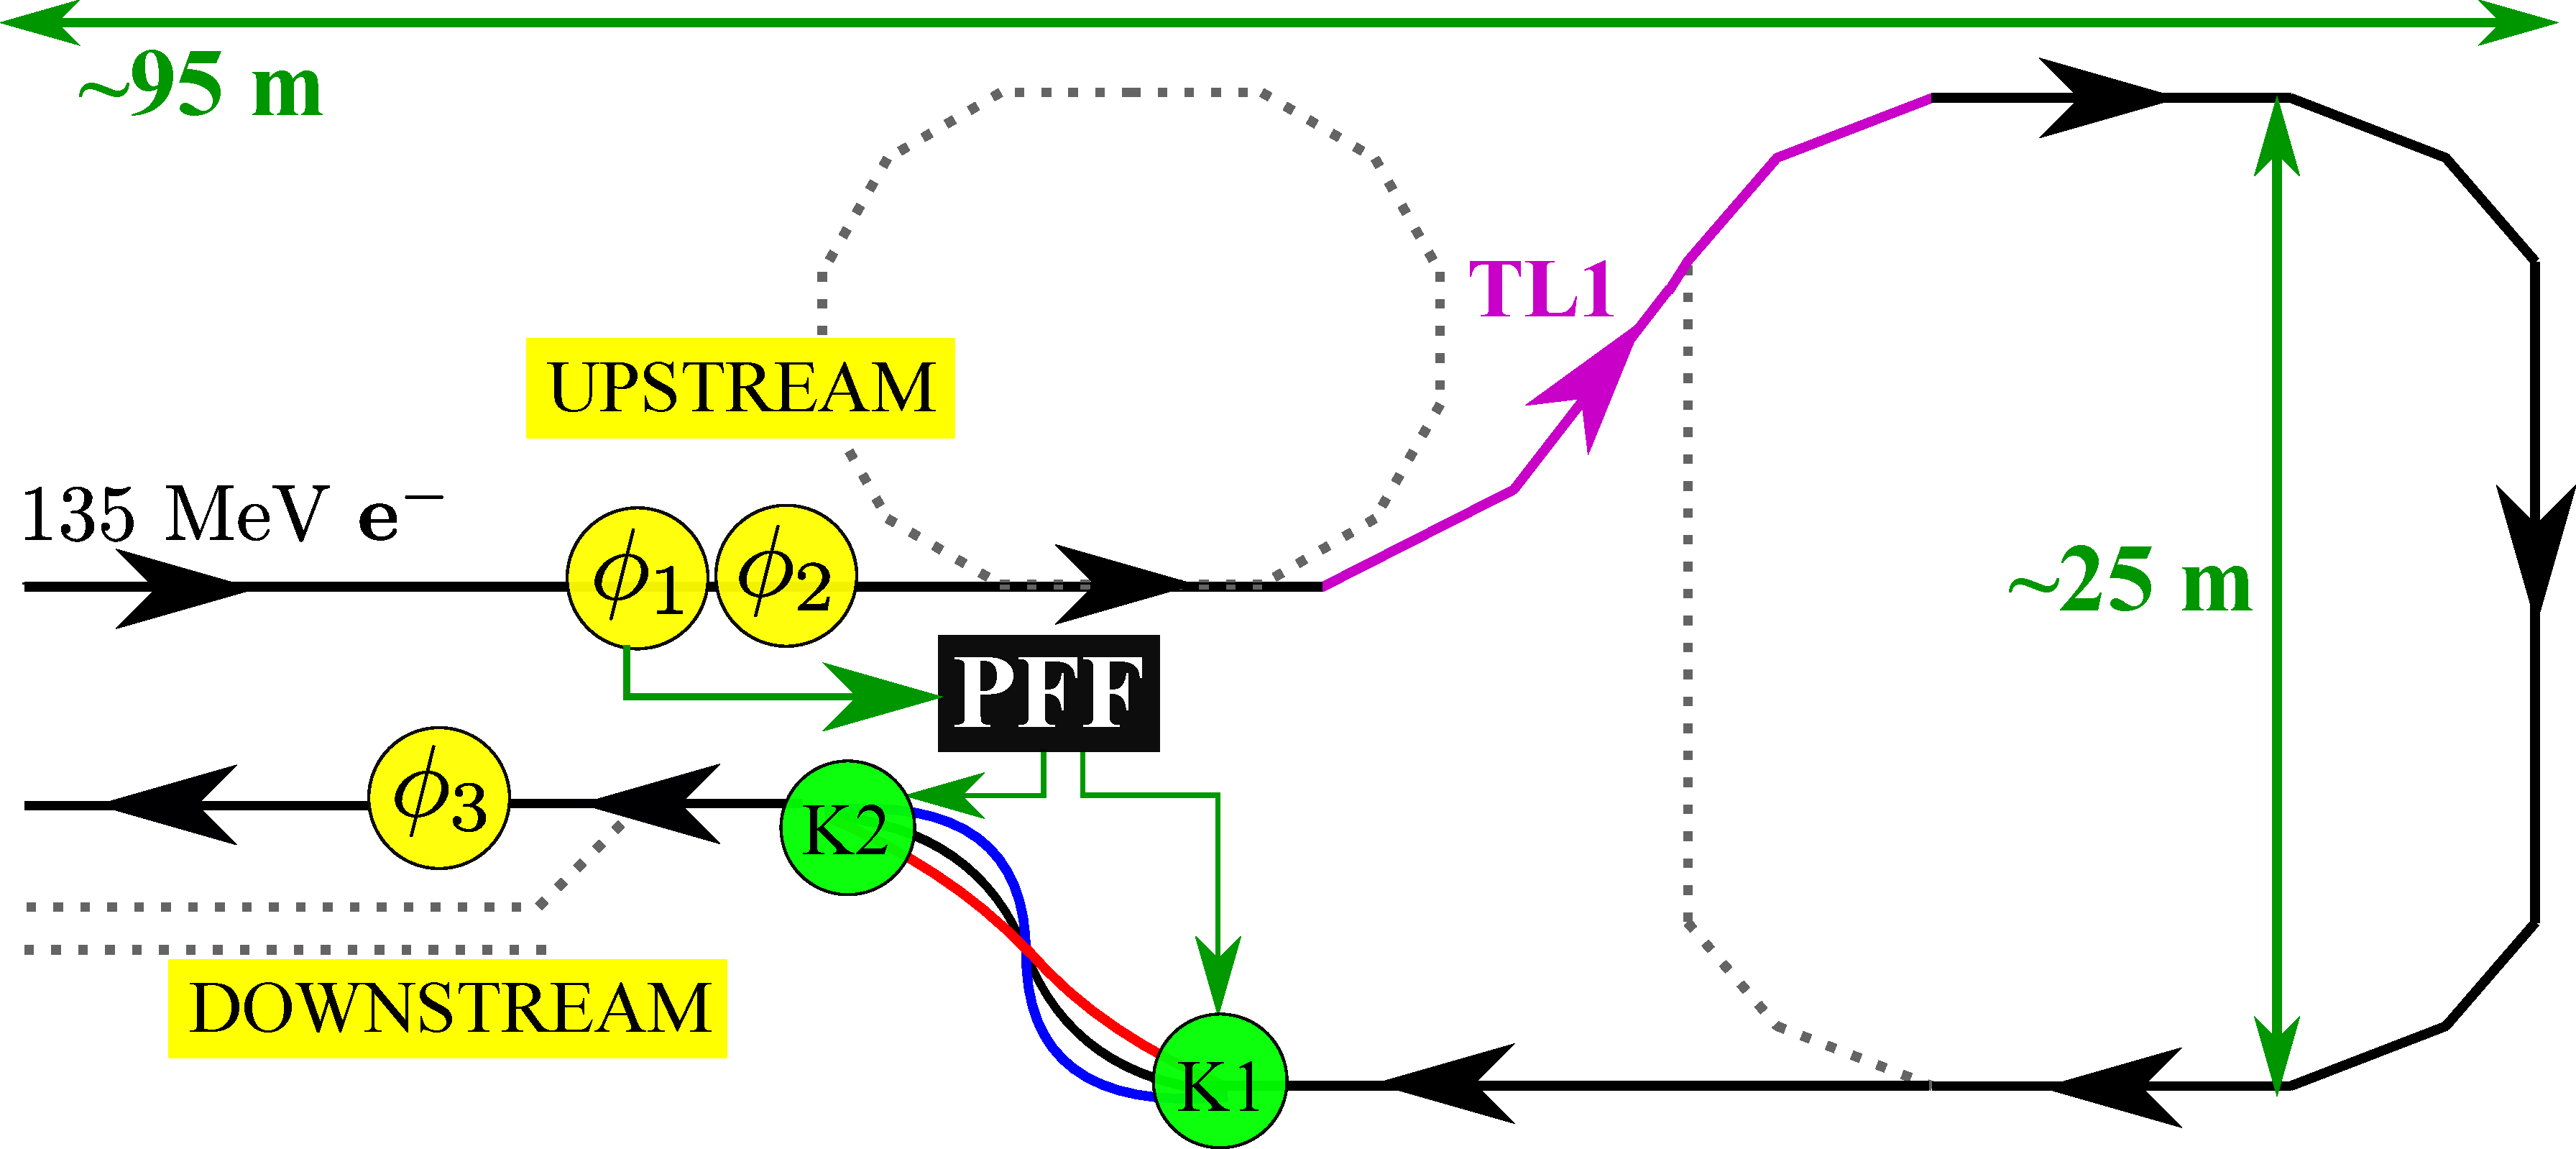
\includegraphics[width=\columnwidth]{ctfpffLayout}% Here is 
  %how to 
  %import EPS art
  \caption{\label{f:pffLayout}Schematic of the PFF prototype at CTF3, 
  showing the phase monitors (\(\phi_1\) , 
  \(\phi_2\) and \(\phi_3\)) and kickers (K1 and K2). The black box “PFF” 
  represents the calculation and output of the correction, including the 
  phase monitor electronics, feedforward controller and kicker amplifiers.
  Dashed lines indicate beam lines that are not used during PFF operation. 
  Bunches arriving early at the upstream monitor (\(\phi_1\)) are directed 
  on to longer trajectories in the correction chicane (blue), and bunches 
  arriving late on to shorter trajectories (red).
    }
\end{figure}


